\section{Case Study Diagnostics}

\begin{figure}[!hbt]
    \centering
    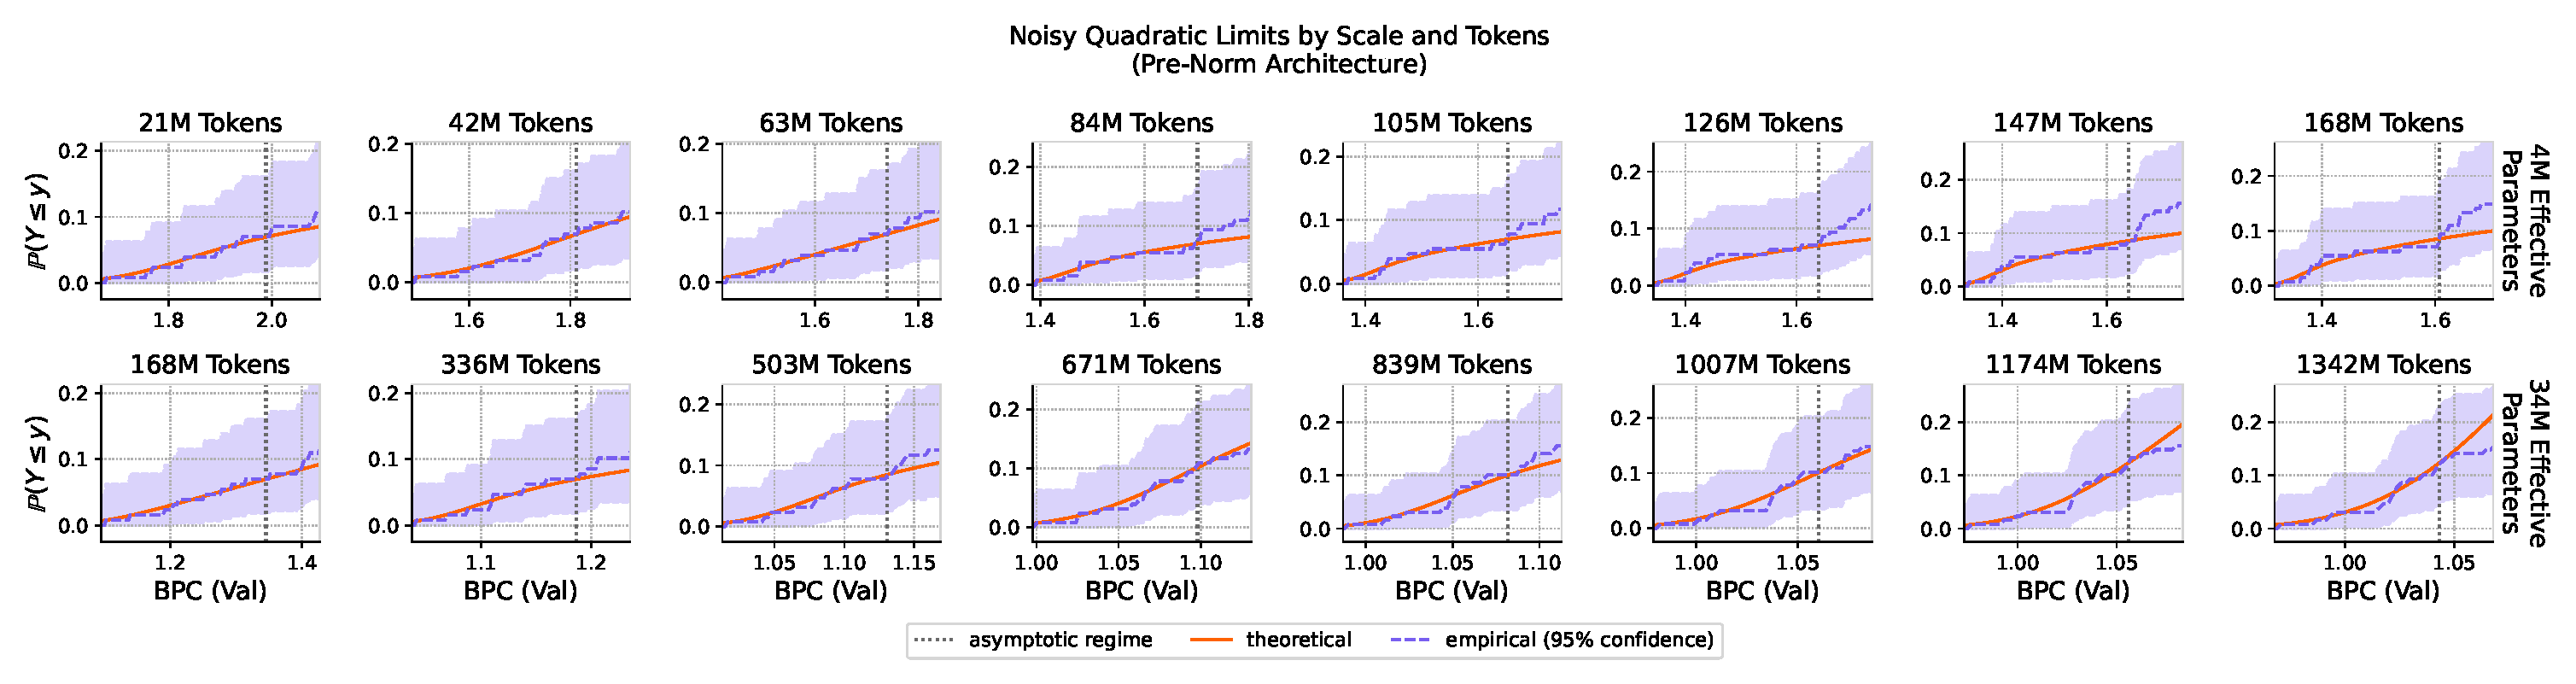
\includegraphics[width=\linewidth]{figures/noisy-quadratic-limit_prenorm-architecture.pdf}
    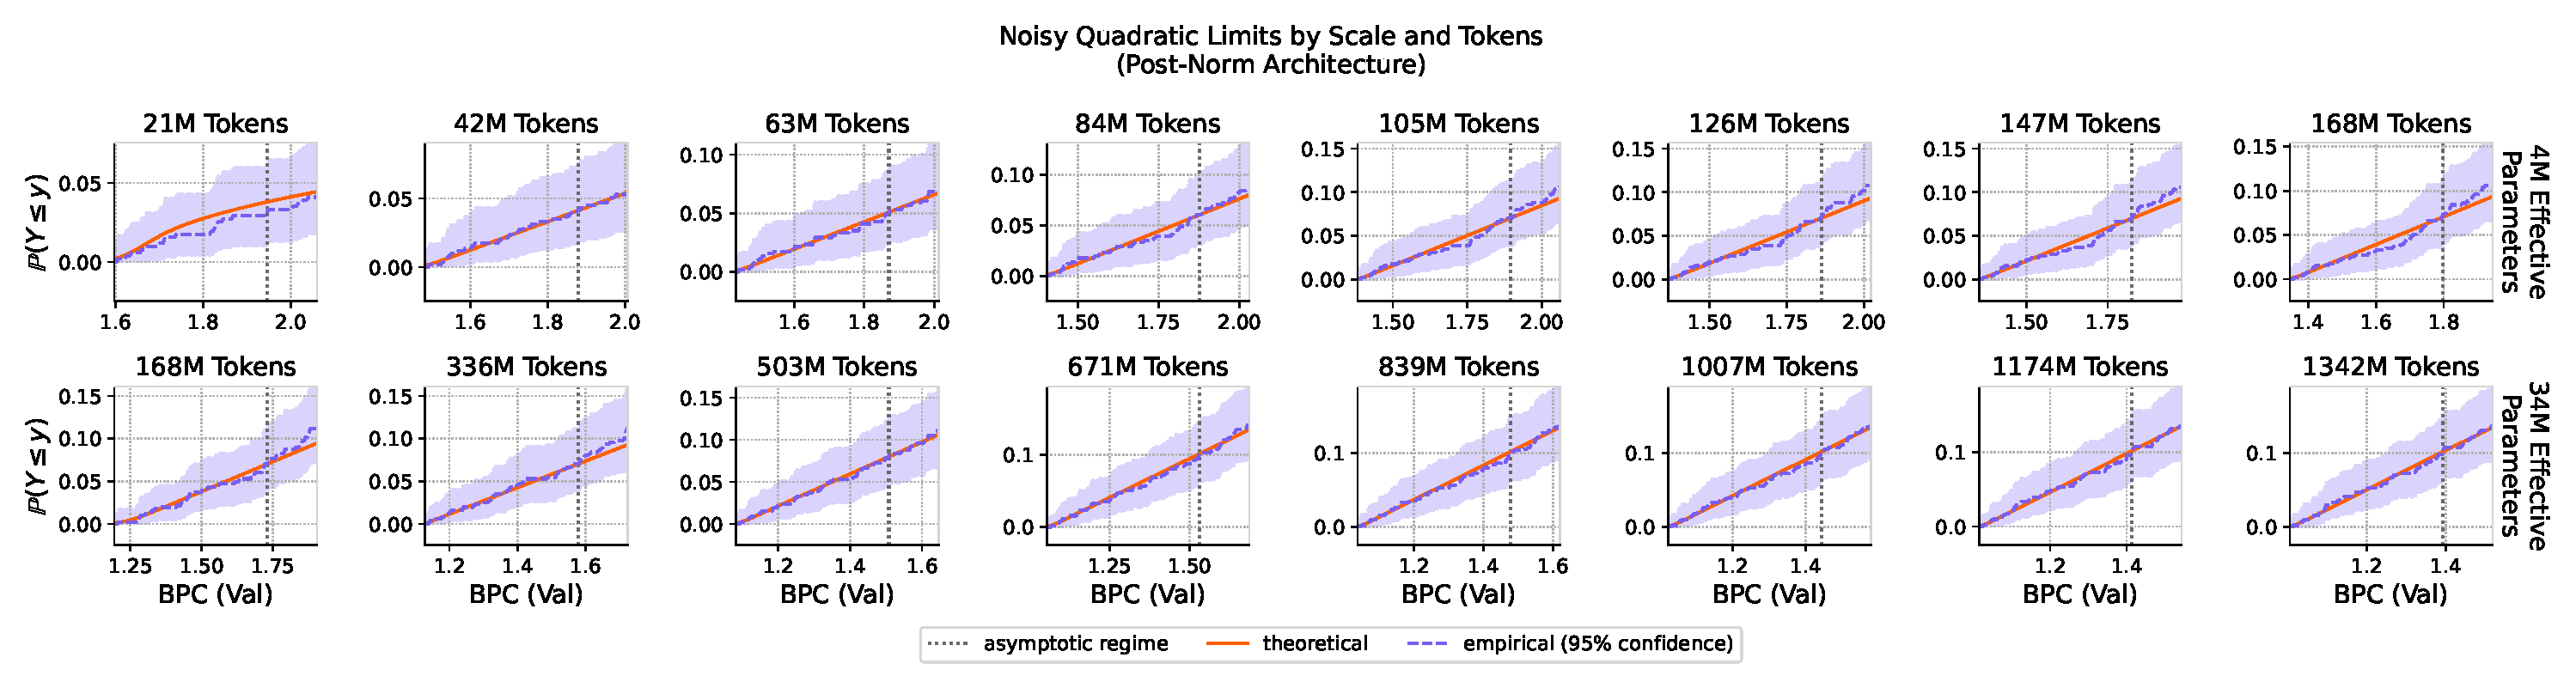
\includegraphics[width=\linewidth]{figures/noisy-quadratic-limit_postnorm-architecture.pdf}
    \caption{
        \emph{The noisy quadratic limit emerges for both architectures, confirming the hyperparameters are well-tuned.} We fit the noisy quadratic to the distribution of validation losses from random search at 4M and 34M parameters for the pre-norm (top) and post-norm (bottom) architectures. The asymptotic regime is smaller for post-norm than pre-norm, an early sign of its hyperparameter sensitivity.
    }
    \label{fig:noisy-quadratic-limit-for-prenorm-vs-postnorm}
\end{figure}
\begin{figure}[!hbt]
    \centering
    \begin{minipage}{0.49\linewidth}
        \centering
        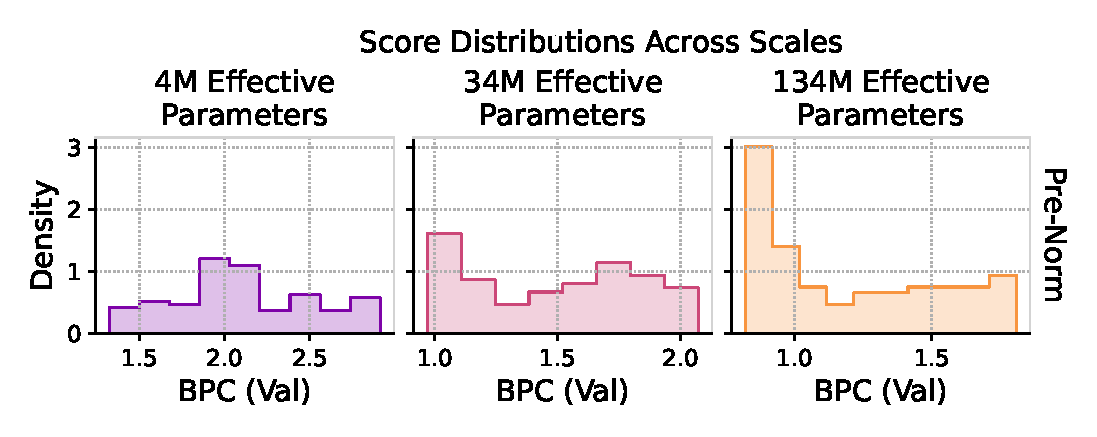
\includegraphics[width=\linewidth]{figures/hyperparameter-sensitivity-across-scales_prenorm-architecture.pdf}
    \end{minipage}
    \hfill
    \begin{minipage}{0.49\linewidth}
        \centering
        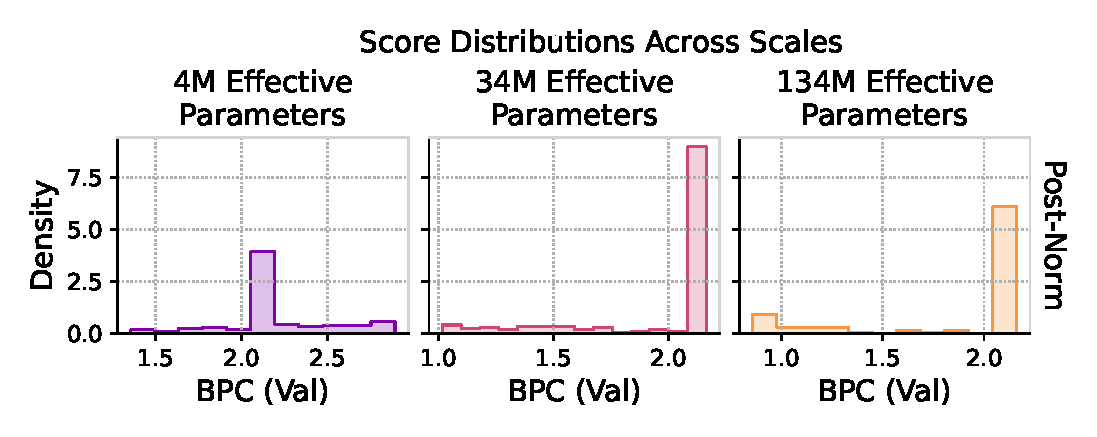
\includegraphics[width=\linewidth]{figures/hyperparameter-sensitivity-across-scales_postnorm-architecture.pdf}
    \end{minipage}
    \caption{
        \emph{Hyperparameter sensitivity decreases with scale for both the pre-norm and post-norm architectures.} Across scales, we compare the score distributions (best 85\%, to exclude divergent runs) for the pre-norm (left) and post-norm (right) architectures. Both place more probability mass near the optimum as scale increases; post-norm, however, maintains a large peak at a suboptimal value, showing persistent tuning difficulty.
    }
    \label{fig:sensitivity-across-scales-for-prenorm-vs-postnorm}
\end{figure}
\begin{figure}[!hbt]
    \centering
    \begin{minipage}{0.49\linewidth}
        \centering
        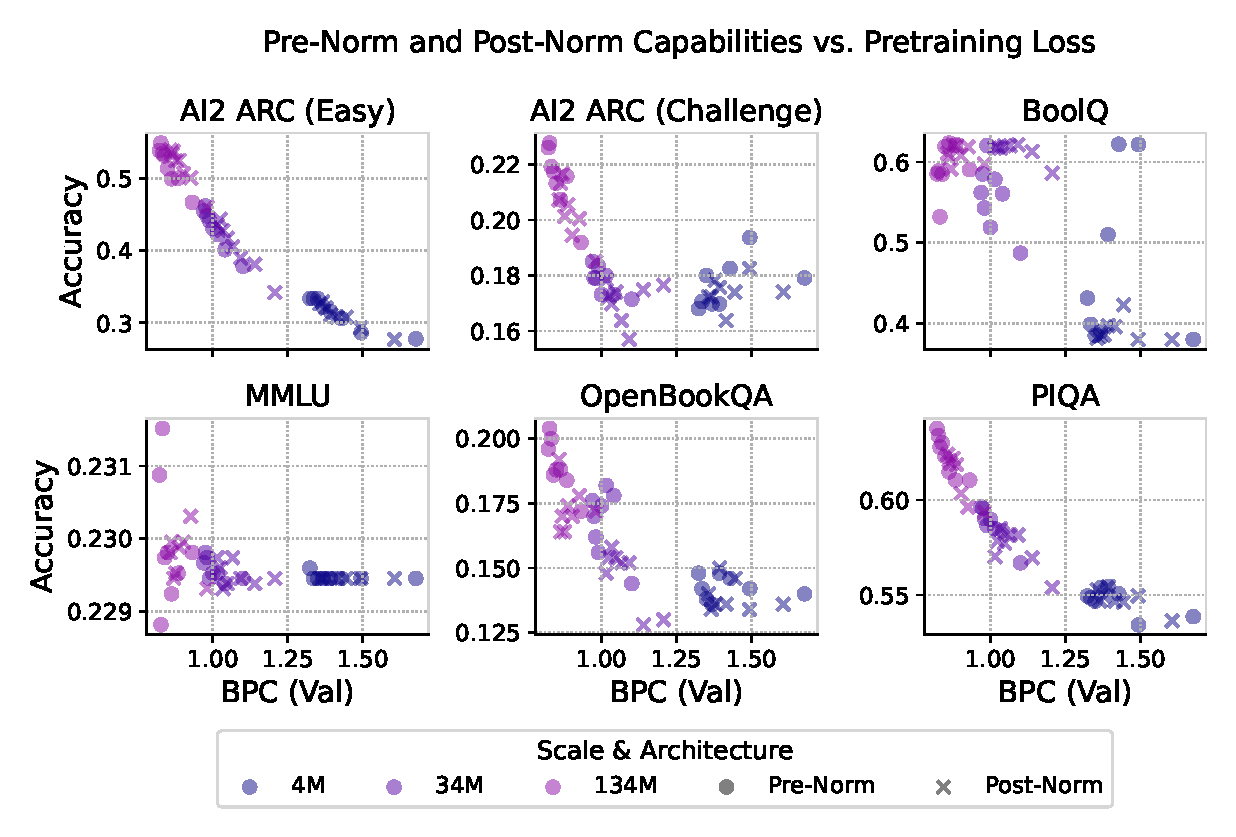
\includegraphics[width=\linewidth]{figures/capabilities-vs-pretraining-loss_prenorm-and-postnorm-architectures.pdf}
        \caption{
            \emph{Pretraining loss corresponds to capabilities both within and across pre-norm and post-norm architectures.} Each panel plots pretraining loss against accuracy for a different task. Across scales and architectures, all points fall on a common trend: equal loss implies equal capability.
        }
        \label{fig:perplexity-capability-correspondence-for-prenorm-vs-postnorm}
    \end{minipage}
    \hfill
    \begin{minipage}{0.49\linewidth}
        \centering
        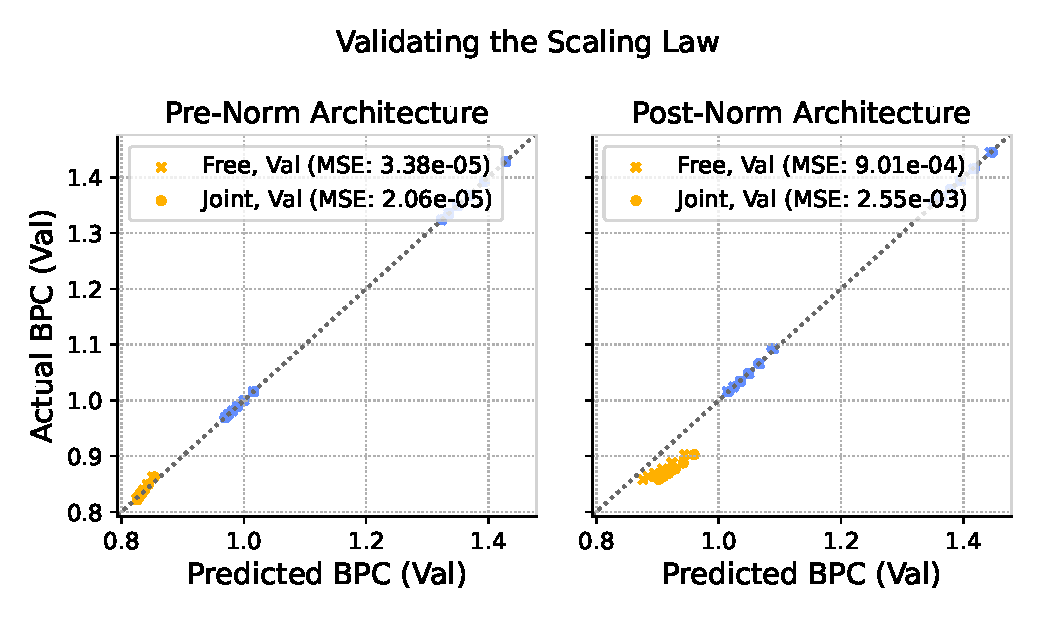
\includegraphics[width=\linewidth]{figures/validating-the-scaling-law.pdf}
        \caption{
            \emph{The scaling laws extrapolate comparably well with free vs. joint irreducible error terms.} We compare sharing the irreducible error term across the architectures (\texttt{joint}) vs. allowing them to differ (\texttt{free}). The pre-norm scaling law extrapolates very well in both cases. The post-norm law extrapolates somewhat, but could likely benefit from even further hyperparameter tuning.
        }
        \label{fig:validating-the-scaling-law}
    \end{minipage}
\end{figure}
\begin{figure}[!hbt]
    \centering
    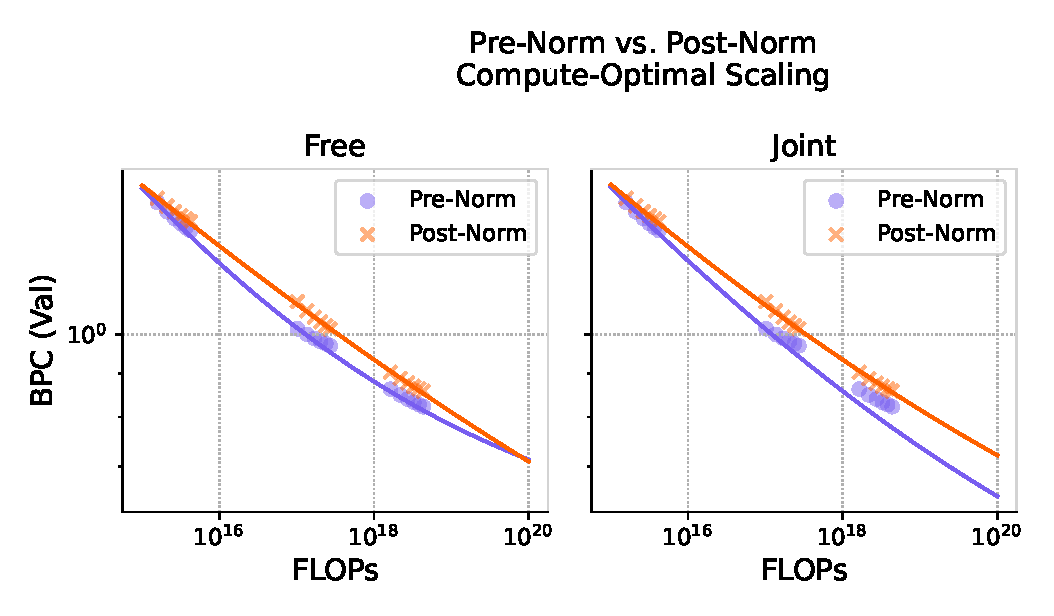
\includegraphics[width=0.6\linewidth]{figures/prenorm-vs-postnorm-compute-optimal-scaling.pdf}
    \caption{
        \emph{Pre-norm scales better than post-norm near the data; far from it, extrapolation reflects the irreducible error.} We fit the scaling laws to all available data and compare them under two conditions: separate (left) vs. shared (right) irreducible errors. Across the range we explore, pre-norm scales better. Outside that range, pre-norm continues to scale better if you believe that both architectures saturate at the same final loss. Under this assumption, the gap grows with compute and we recover the large-scale advantage of pre-norm from our small-scale experiments.
    }
    \label{fig:prenorm-vs-postnorm-compute-optimal-scaling}
\end{figure}
